\begin{figure}

\begin{center}
\begin{subfigure}[b]{\linewidth}
\begin{minipage}{0.5\linewidth}

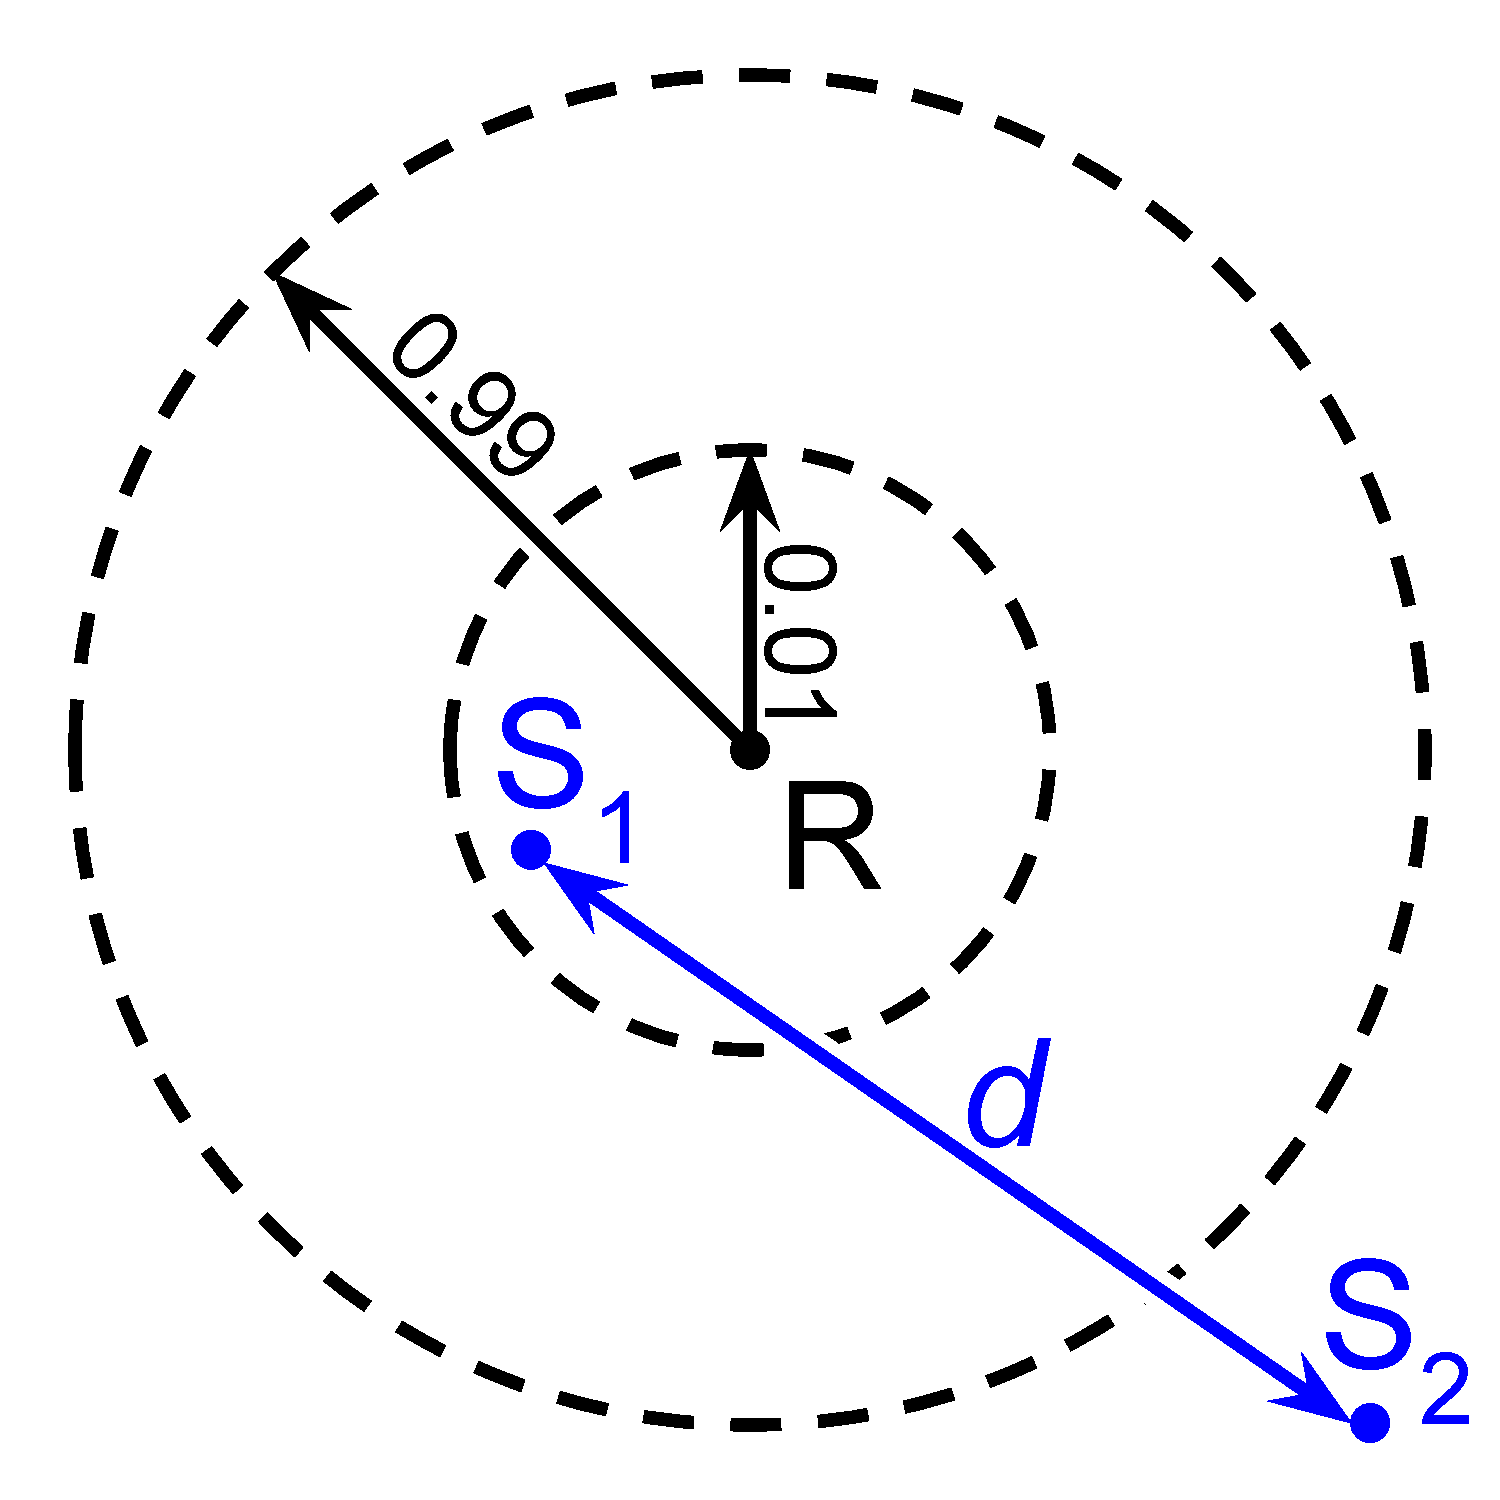
\includegraphics[width=0.75\linewidth]{img/elasticity-statistic}

\end{minipage}
\begin{minipage}{0.5\linewidth}
\caption{
A schematic depicting the process used to generate the dissimilarity statistic for each metric.
}
\label{fig:dissimilarity_statistic}
\end{minipage}

\end{subfigure}

\begin{subfigure}[b]{\linewidth}
\begin{minipage}{0.6\linewidth}
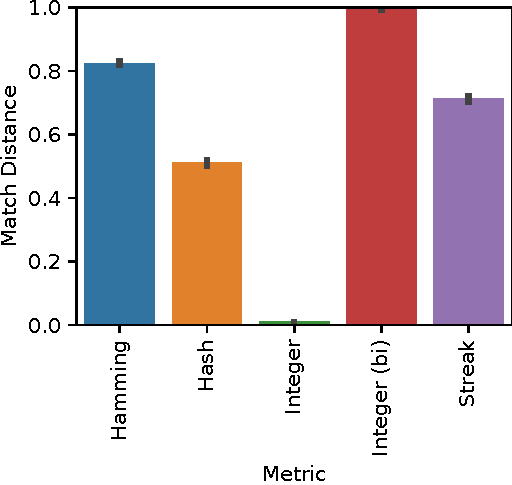
\includegraphics[width=\linewidth]{img/sphere_reverse/bitweight=0dot5+seed=1+title=dimensionality_barplot+_data_hathash_hash=93f97a11cb443d35+_script_fullcat_hash=03ce1e318a24a109+ext=}
\end{minipage}
\begin{minipage}{0.35\linewidth}
\caption{
Mean statistic values for each metric.
Error bars represent 95\% confidence intervals.
}
\label{fig:sphere_reverse_distnplot}
\end{minipage}
\end{subfigure}
s
\begin{subfigure}[b]{\columnwidth}
\centering
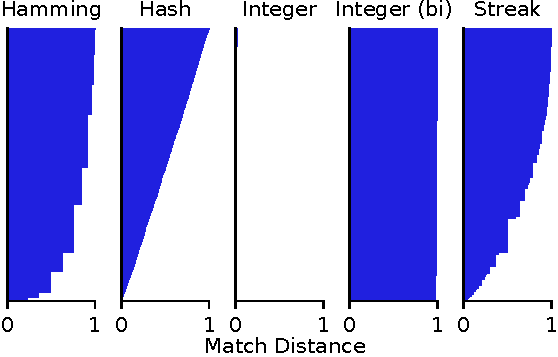
\includegraphics[width=\columnwidth]{img/sphere_reverse/bitweight=0dot5+seed=1+title=dimensionality_distnplot+_data_hathash_hash=93f97a11cb443d35+_script_fullcat_hash=03ce1e318a24a109+ext=}
\caption{
Statistic distribution, where each horizontal bar sliver represents one independent observation.
}
\label{fig:sphere_reverse_barplot}
\end{subfigure}

\caption{
Dissimilarity constraint of tag-matching metrics.
}
\label{fig:sphere_reverse}

\end{center}
\end{figure}
